\chapter{Results}
\label{chap:results}


Spatially and spectrally resolved line emission was detected for CO (3-2), HCO$^{+}$ (4-3), HCN (4-3), and CS (7-6) across around 50 channels with velocity resolution of 0.42 km s$^{-1}$. Here we present a discussion of these data, including line-emission statistics, diagnostic plots, and a consideration of the cloud contamination present.


\section{Cloud Contamination}
\label{section:cloud_contamination}
% Ex footnote: \texttt{K2Phot}\footnote{\href{https://github.com/vincentvaneylen/k2photometry}{https://github.com/vincentvaneylen/k2photometry}} \citep{vaneylen2016}

Cloud contamination occurs when emission from gas clouds along the observation's line of sight is detected. This is typically not a significant issue for observations of protoplanetary disks in low-mass star forming regions (SFRs), but since the Orion Nebula has a signicantly higher gas density than those low-mass SFRs, cloud contamination presents problems in these data. This is particularly evident in the CO line, thanks to its low critical density and relatively high abundance in the background clouds, which allows it to excite and emit more readily than other molecules. As a result of higher critical densities and lower abundances, cloud contamination is less significant, but still present, in the other lines. It is crucial to manage and minimize the effects of this contamination before modeling so that our fitting algorithms do not try to model the cloud emission.

% You’ll need to explain why we want to minimize rms noise: normally, removing data should increase rms noise (because rms noise should decrease as the square root of the number of data points).  However, when we remove short baselines we see exactly the opposite, which tells us that there is signal on the short baselines (from the cloud) causing the off-source rms to be artificially inflated.  We look for the inflection point where the plot goes from decreasing rms noise to increasing rms noise, because that tells us that noise statistics are starting to dominate over cloud contamination. 



Luckily, there exist ways to minimize the effects of cloud contamination. An obvious way to do this would be to simply crop out the contaminated regions; however, since we model in the visibility domain (a Fourier transform away from the image domain), we are unable to separate the cloud contamination by physical location, like we could in an image. Instead, we take advantage of the fact that the contaminating clouds tend to be very large relative to a proplyds and that, as discussed in \S\ref{chap:introduction}, interferometers have the ability to filter by length scale. Using these two features, we may exclude a selection of the shortest baselines used in our data, effectively shrinking the largest angular scales to which our receivers are sensitive. This, in turn, significantly reduces the effects of the cloud emission, since those short baselines that are recording the noise are also too short to be recording meaningful information about the disk\footnote{This can be shown with a quick calculation of the angular resolution of the short baselines. We can easily consider the angular resolution of a 40\,k\lambda baseline: $\theta = \lambda/D = 1/(40\,000)$ radians $\gtrapprox$ 5''. At Orion's distance of 389 pc, this corresponds to $\sim$2000 au, larger than the $\sim$2'' (\textless800 au) that our disks span.}.


To characterize the cloud contamination in our images, we iteratively remove more and more of the shortest baselines from our data and measure the resulting RMS noise of an off-source area at each step. Were there no cloud contamination, this plot of RMS vs. min-baseline would trend upwards (following the fact that noise is typically proportional to the inverse square root of amount of data). However, we can recognize the signature of cloud contamination if we find unexpectedly high noise at low baselines that falls off at longer ones. This decrease reflects the fact that, since the clouds are large, only the shortest baselines are sensitive to their emission. This indicates that the optimal value to use as our minimum baseline length would be the inflection point at which the cloud contamination's contribution (decreasing with baseline length) gives way to the normal losses that come with decreasing signal (increasing with baseline length). The results of making such plots are shown in Fig. \ref{fig:noise-profiles}.

From these plots, we find that excluding baselines less than 110 k$\lambda$, 80 k$\lambda$, and 60  k$\lambda$ for HCO$^{+}$, HCN, and CO, respectively, yielded optimum results. Since emission from the CS line already has a very low SNR and a higher critical density than the clouds can easily access, it showed minimal contamination and thus excluding baselines did not improve the observations. Image statistics resulting from these cuts are presented in Table \ref{tab:baseline_cutting_table}.

% Calculations for this are made in scratch_02.py but maybe should be in scratch_03 now.


\begin{figure}[t]
  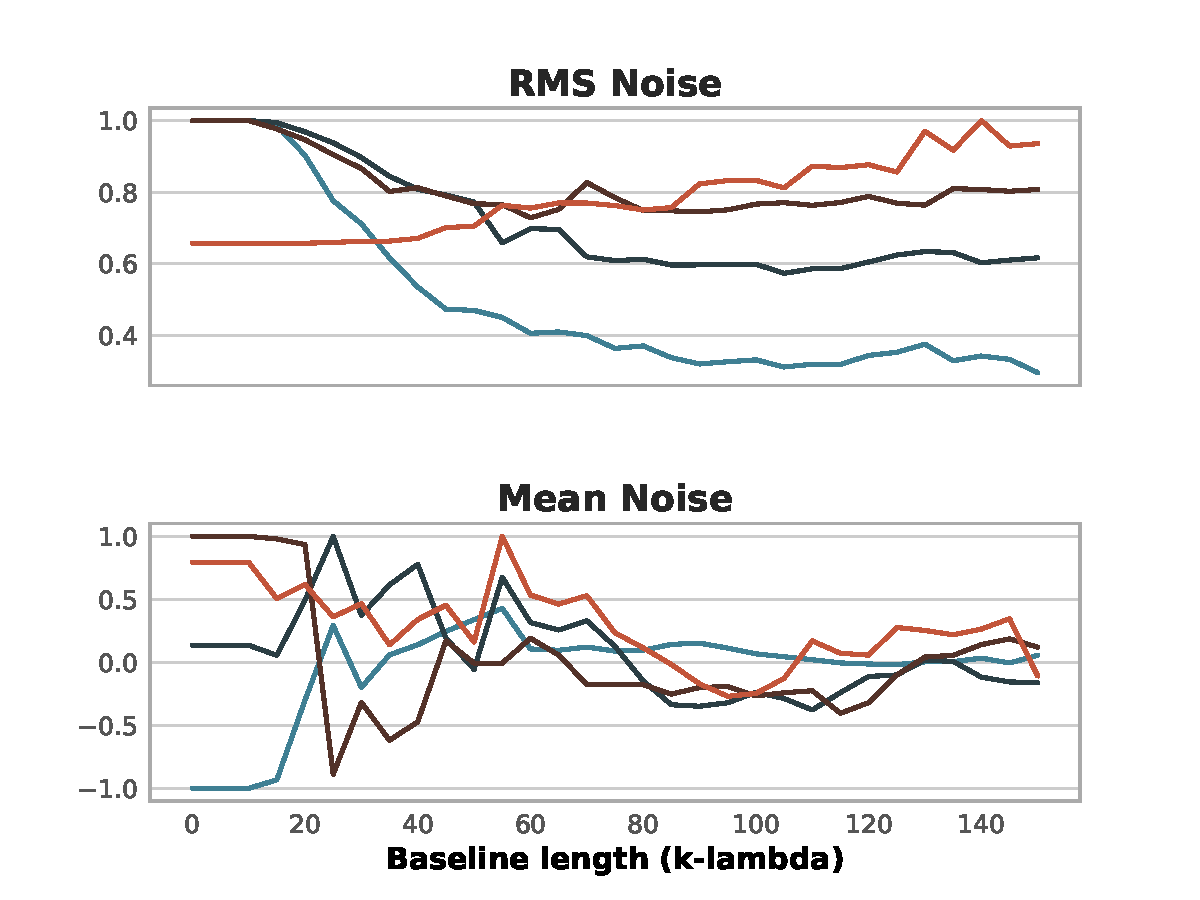
\includegraphics[width=\linewidth]{full_baseline_analysis.pdf}%
  \caption{Noise profiles as a function of minimum baseline length for the four molecular lines in our dataset. Dashed lines represent optimal cut locations, at the minimum where cloud contamination is noise that is introduced from removing data is not yet too large. Since CS (dotted line) has no cloud contamination, we do not remove any baselines from it. Quantitative results from this process are summarized in Table \ref{tab:baseline_cutting_table}.}
  \label{fig:noise_profiles}
\end{figure}





\section{Line Data}
\label{section:line_data}

Integrated line flux was measured using the Miriad task \texttt{cgcurs} to measure the total flux in a zeroth moment map over the region enclosed by the 3$\sigma$ contour. Due to the disks' overlap and interaction with one another, defining the disks' boundaries, and consequently where to place the bounding box for flux-integration, is not entirely clear. This introduces a significant source of uncertainty in the calculation of total disk flux, as noted in \citet{Williams2014}, which they estimate to be around 30\%. The results of these measurements are shown in Table \ref{tab:baseline_cutting_table}. From these values, we may estimate the disks' gas masses.


\begin{table}
  \begin{threeparttable}
    \centering
    \caption{Integrated Flux Measurements with Baseline Cuts}
    \label{tab:baseline_cutting_table}
    \renewcommand{\arraystretch}{1.2}
    \begin{tabular}{l | c | c | c  c }
      \toprule \toprule
      {Molecular}     & Baselines       & Max Angular & \multicolumn{2}{c}{Integrated Line Flux (Jy km s$^{-1}$)} \\
      Line            & Included        & Scale ('')  & Disk A        & Disk B \\
      \midrule %\midrule
      CO (3-2)        & All             & 8.4        & \tnote{*}      &  \tnote{*} \\
      CO (3-2)        & $>60 k\lambda$  & 3.4        & 2.58$\pm$0.47  & 1.85 $\pm$ 0.39 \\
      HCN (4-3)       & All             & 8.2        & 0.80$\pm$0.07  &  0.26 $\pm$ 0.08 \\
      HCN (4-3)       & $>80 k\lambda$  & 2.6        & 0.69$\pm$0.05  &  0.17 $\pm$ 0.08 \\
      HCO$^{+}$ (4-3) & All             & 8.2        & 5.79$\pm$0.49  &  2.29 $\pm$ 0.56 \\
      HCO$^{+}$ (4-3) & $>110 k\lambda$ & 1.9        & 4.15$\pm$0.31  &  0.80 $\pm$ 0.22 \\
      CS (7-6)        & All             & 8.5        & 0.024$\pm$0.02 & [no detection] \\
      \bottomrule
    \end{tabular}
    \begin{tablenotes}\footnotesize
      \item[*]
      \item[**] Integrated line intensity was not calculated for CO(3-2) before the baseline cuts, as the data were too contaminated to give meaningful results.
    \end{tablenotes}
  \end{threeparttable}
\end{table}



% Results from tools.py/get_int_line_flux()
% HCO+, >110: 0.62,
% HCO+, all: 0.80, 5.79(0.488), 2.287(0.561)
% CO, all: 0.51: unusable
% CO, >60: 0.495, 2.579(0.472), 1.855(0.391)
% HCN, all: 0.161, 0.797(0.0673), 0.255(0.077879)
% HCN, >80, 0.132, 0.690(0.0487), 0.170(0.0775)
% CS, all: 0.023, 0.0242(0.0246), NA





Assuming optically thin emission and Local Thermodynamic Equilibrium (LTE), the line-emitting gas mass, M$_{\text{gas}}$ is given by:

\begin{align}
  M_{\text{gas}}= \frac{4 \pi}{h \nu_0} \frac{F m d^2}{A_{ul} X_u},
  \label{M_gas}
\end{align}

where $F$ is the integrated line flux, $m$ is the mass of the emitting gas molecule, $d$ is the distance to the source, $h$ is the Planck constant, $\nu_0$ is the molecular line's rest frequency, $A_{ul}$ is the Einstein coefficient for the ($u - l$) transition, and

\begin{align}
  X_u = \frac{N_u}{N_{\text{tot}}} = (2 J_u + 1) \frac{\exp [-B_0 J_u (J_u + 1) h c/kT_{\text{ex}}]}{kT_{\text{ex}}/hc B_0}.
  \label{X_u}
\end{align}

In Eqn. \ref{X_u}, $\frac{N_u}{N_{\text{tot}}}$ is the ratio of the number of molecules in the upper state to the total number of molecules; the values used for this measurement and descriptions of them are given in Table \ref{tab:mass_calc_vals}. %Since Eqn. \ref{M_gas} is the mass of the observed gas species, it must be scaled by the its relative abundance (fit for in Section 4) to obtain a total mass.


\begin{table}
  \centering
  \begin{threeparttable}
    \caption{Values Used in Gas Mass Calculation (for \hco(4-3))}
    \label{tab:mass_calc_vals}
    \renewcommand{\arraystretch}{1.2}
    \begin{tabular}{l | c | c | c }
      \toprule \toprule
      Parameter            & Value   & Description         & Source  \\
      \midrule %\midrule
      F ($\frac{\text{erg Hz}}{\text{cm$^2$ s Hz}}$) & $6.8 \times 10^{-12}$ & Integrated line flux     &  0 \\
      $\nu_0$ (GHz)         & 356.73 & Rest frequency & \citet{Schoier2005} \\
      J                     & 4      & Quantum number of upper level & \\
      A$_{4-3}$ (s$^{-1}$)  & $3.63 \times 10^{-3}$  & Einsten A coefficient    & \citet{Schoier2005}  \\
      % E$_{4-3}$ (cm$^{-1}$) & 29.75  & Energy of 4-3 transition & \citet{Schoier2005} \\
      B$_0$ (cm$^{-1}$)     & 0.187  & Rotational constant      & 1 \\
      T$_\text{ex}$         & 17     & Excitation Temperature   & \citet{Factor2017}  \\
      $d$ (pc)              & 389    & Distance & \cite{GaiaCollaboration2018}  \\
      $m$ (g)               & $\frac{29}{6 \times 10^{23}}$ & Mass of molecule & \citet{Schoier2005}, converted to $g$ \\
      \bottomrule
    \end{tabular}
    \begin{tablenotes}\footnotesize
      \item[0] Calculated with MIRIAD task \texttt{cgcurs}
      \item[1] B$_0 = \frac{2 \pi E_{4-3}}{h c)} \rightarrow B_o (hc) = 2\pi E_{4-3}$ (the formula for converting an electromagnetic wave's energy into a wavenumber), where E0 = 0.0297 cm$^{-1}$
    \end{tablenotes}
  \end{threeparttable}
\end{table}

Plugging these values in, we find a disk mass of $M_\text{gas}$ = 1.13 M$_\odot$. This is too big, but closer.



% REWORK: Replot m0 and m1 maps to get the text on top.
We now turn to visualizing our data. Since line emission has a third (spectral) dimension, visualizing it presents a unique opportunity and challenge. Moment maps offer us an intuitive way to flatten the three-dimensional data-cube (in $\alpha, \delta, v$) into two dimensions. Moment 0 maps integrate flux along the velocity axis as a function of position, providing insight into structures of emission intensity in the disk's morphology (while essentially sacrificing the data's spectral information), while moment 1 maps, a velocity-weighted intensity integration across position, tell us about a source's velocity gradients. Fig. \ref{fig:baseline_cuts} show zeroth- and first-moment maps, respectively, of emission from the CO, \hco, and HCN lines, with and without short baselines (as defined in Table \ref{tab:baseline_cutting_table}) removed (right and left, respectively)).



With moment maps, we flatten through the velocity axis, but we can also flatten through the spatial dimensions as well using a position-velocity diagram (PVD). PVDs allow us to directly observe the velocity dispersion along a given axis in the image; usually this is a disk's major axis. In Fig. \ref{fig:pv_diag}, we show a PVD of disk A's \hco emission. In it, we see some noticeable asymmetry, both in terms of centroid intensity and in the extra feature at the eastern side of the map, which is likely the tail of disk B.


% MOMENT MAPS
\begin{figure}[h]
  \hspace*{\fill}%
  \subcaptionbox{}{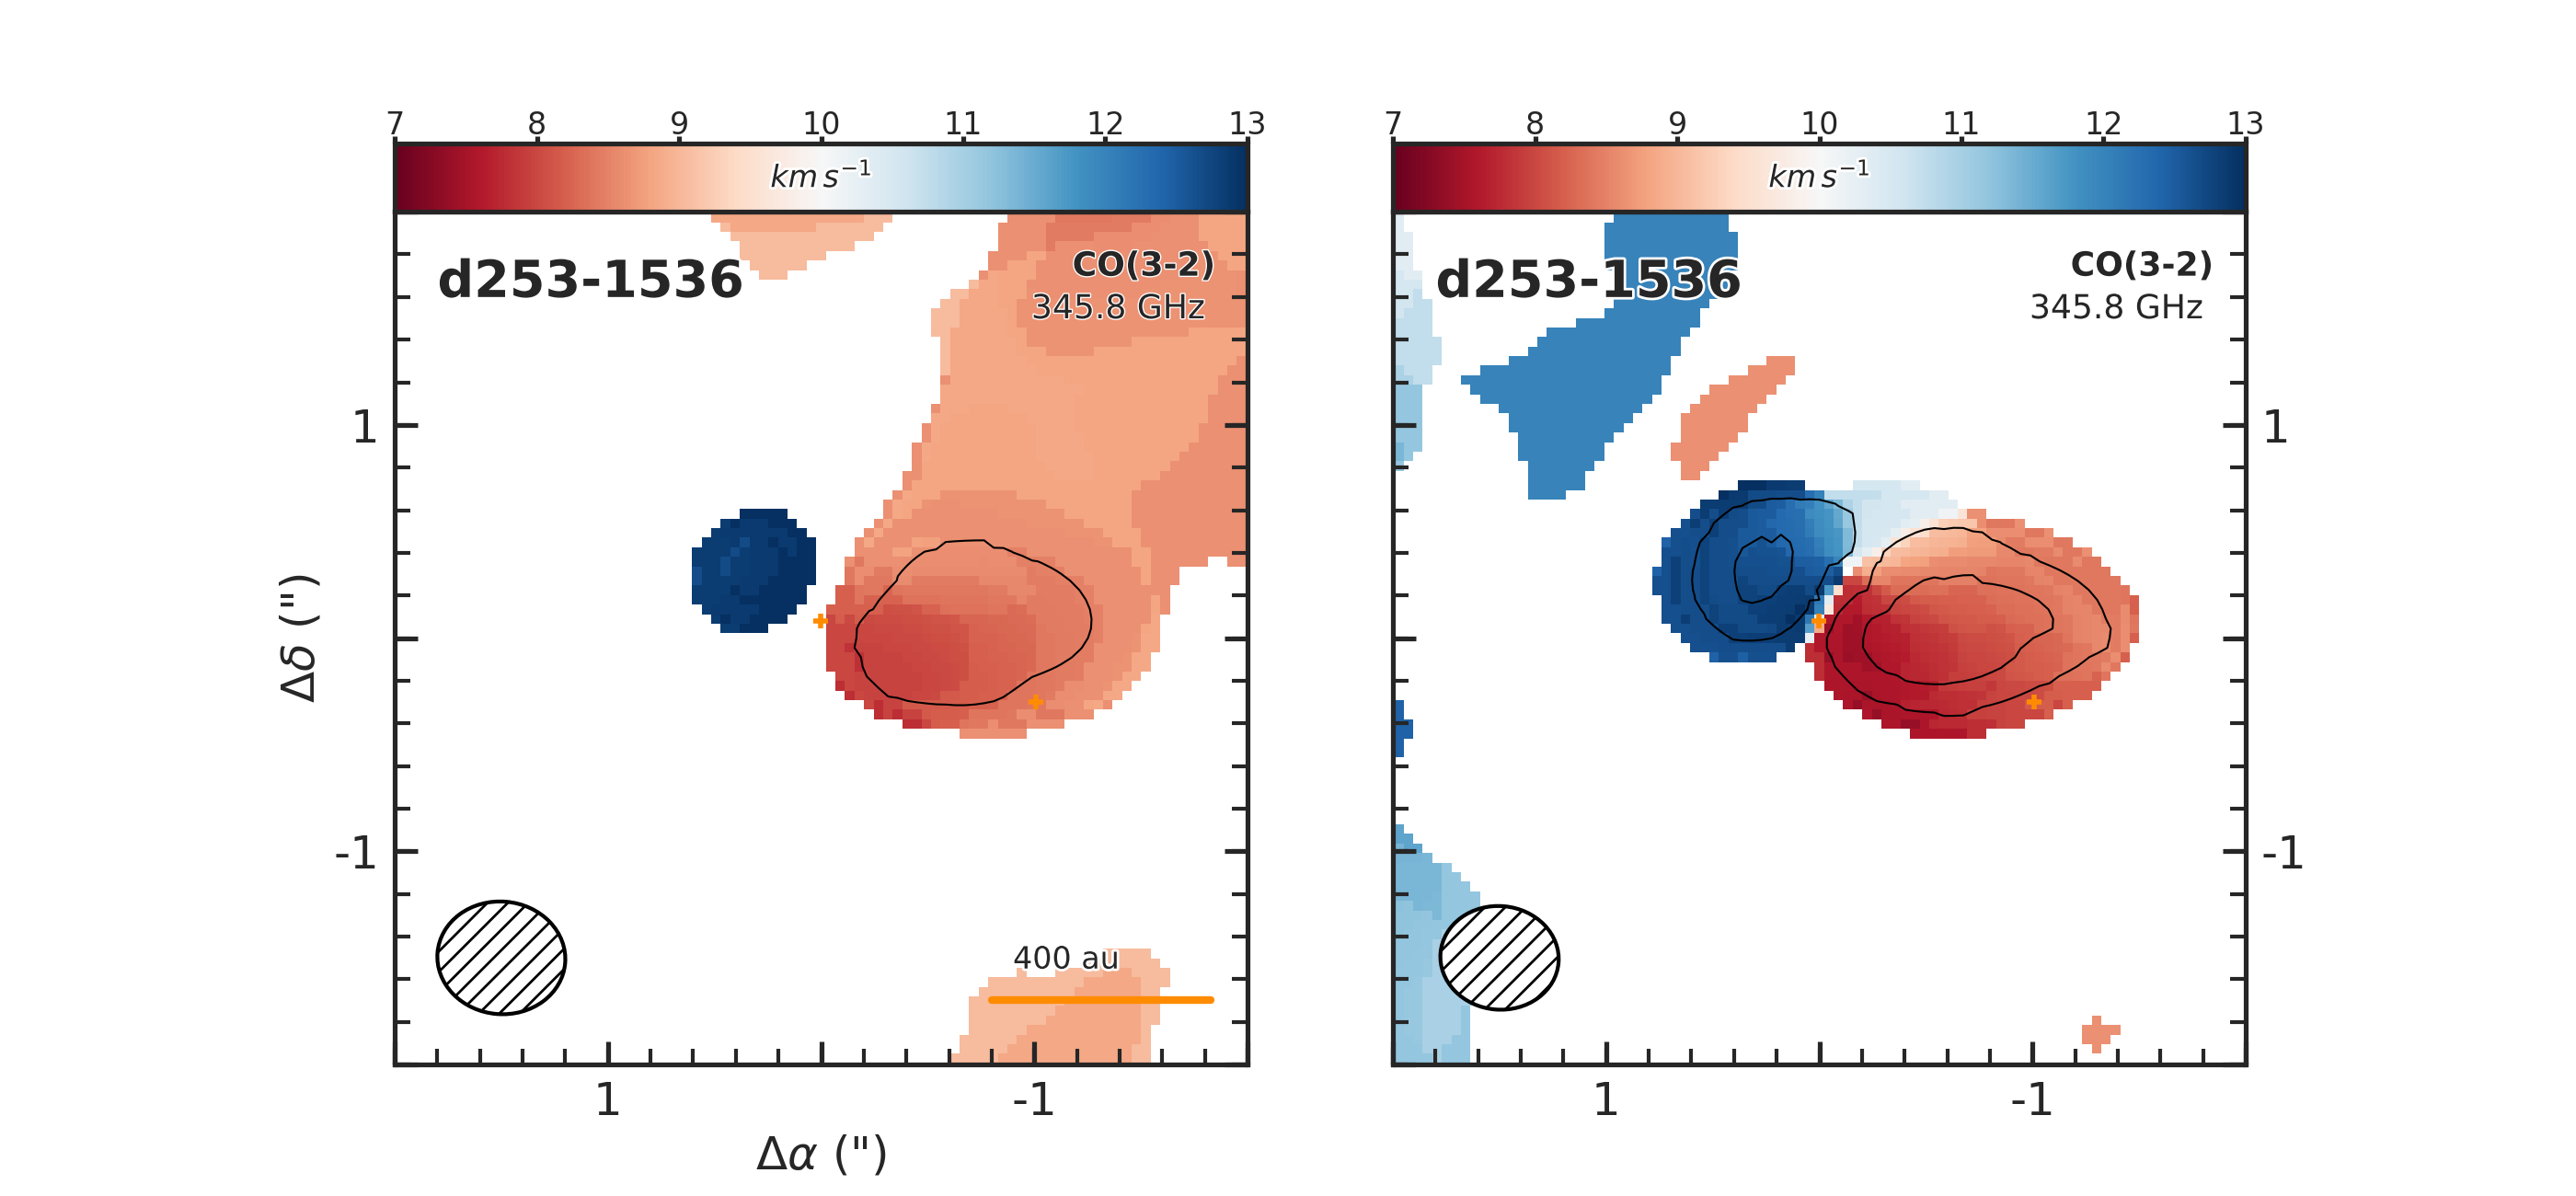
\includegraphics[width=\linewidth]{moment1_co-baselines.pdf}}\vfill%
  \subcaptionbox{}{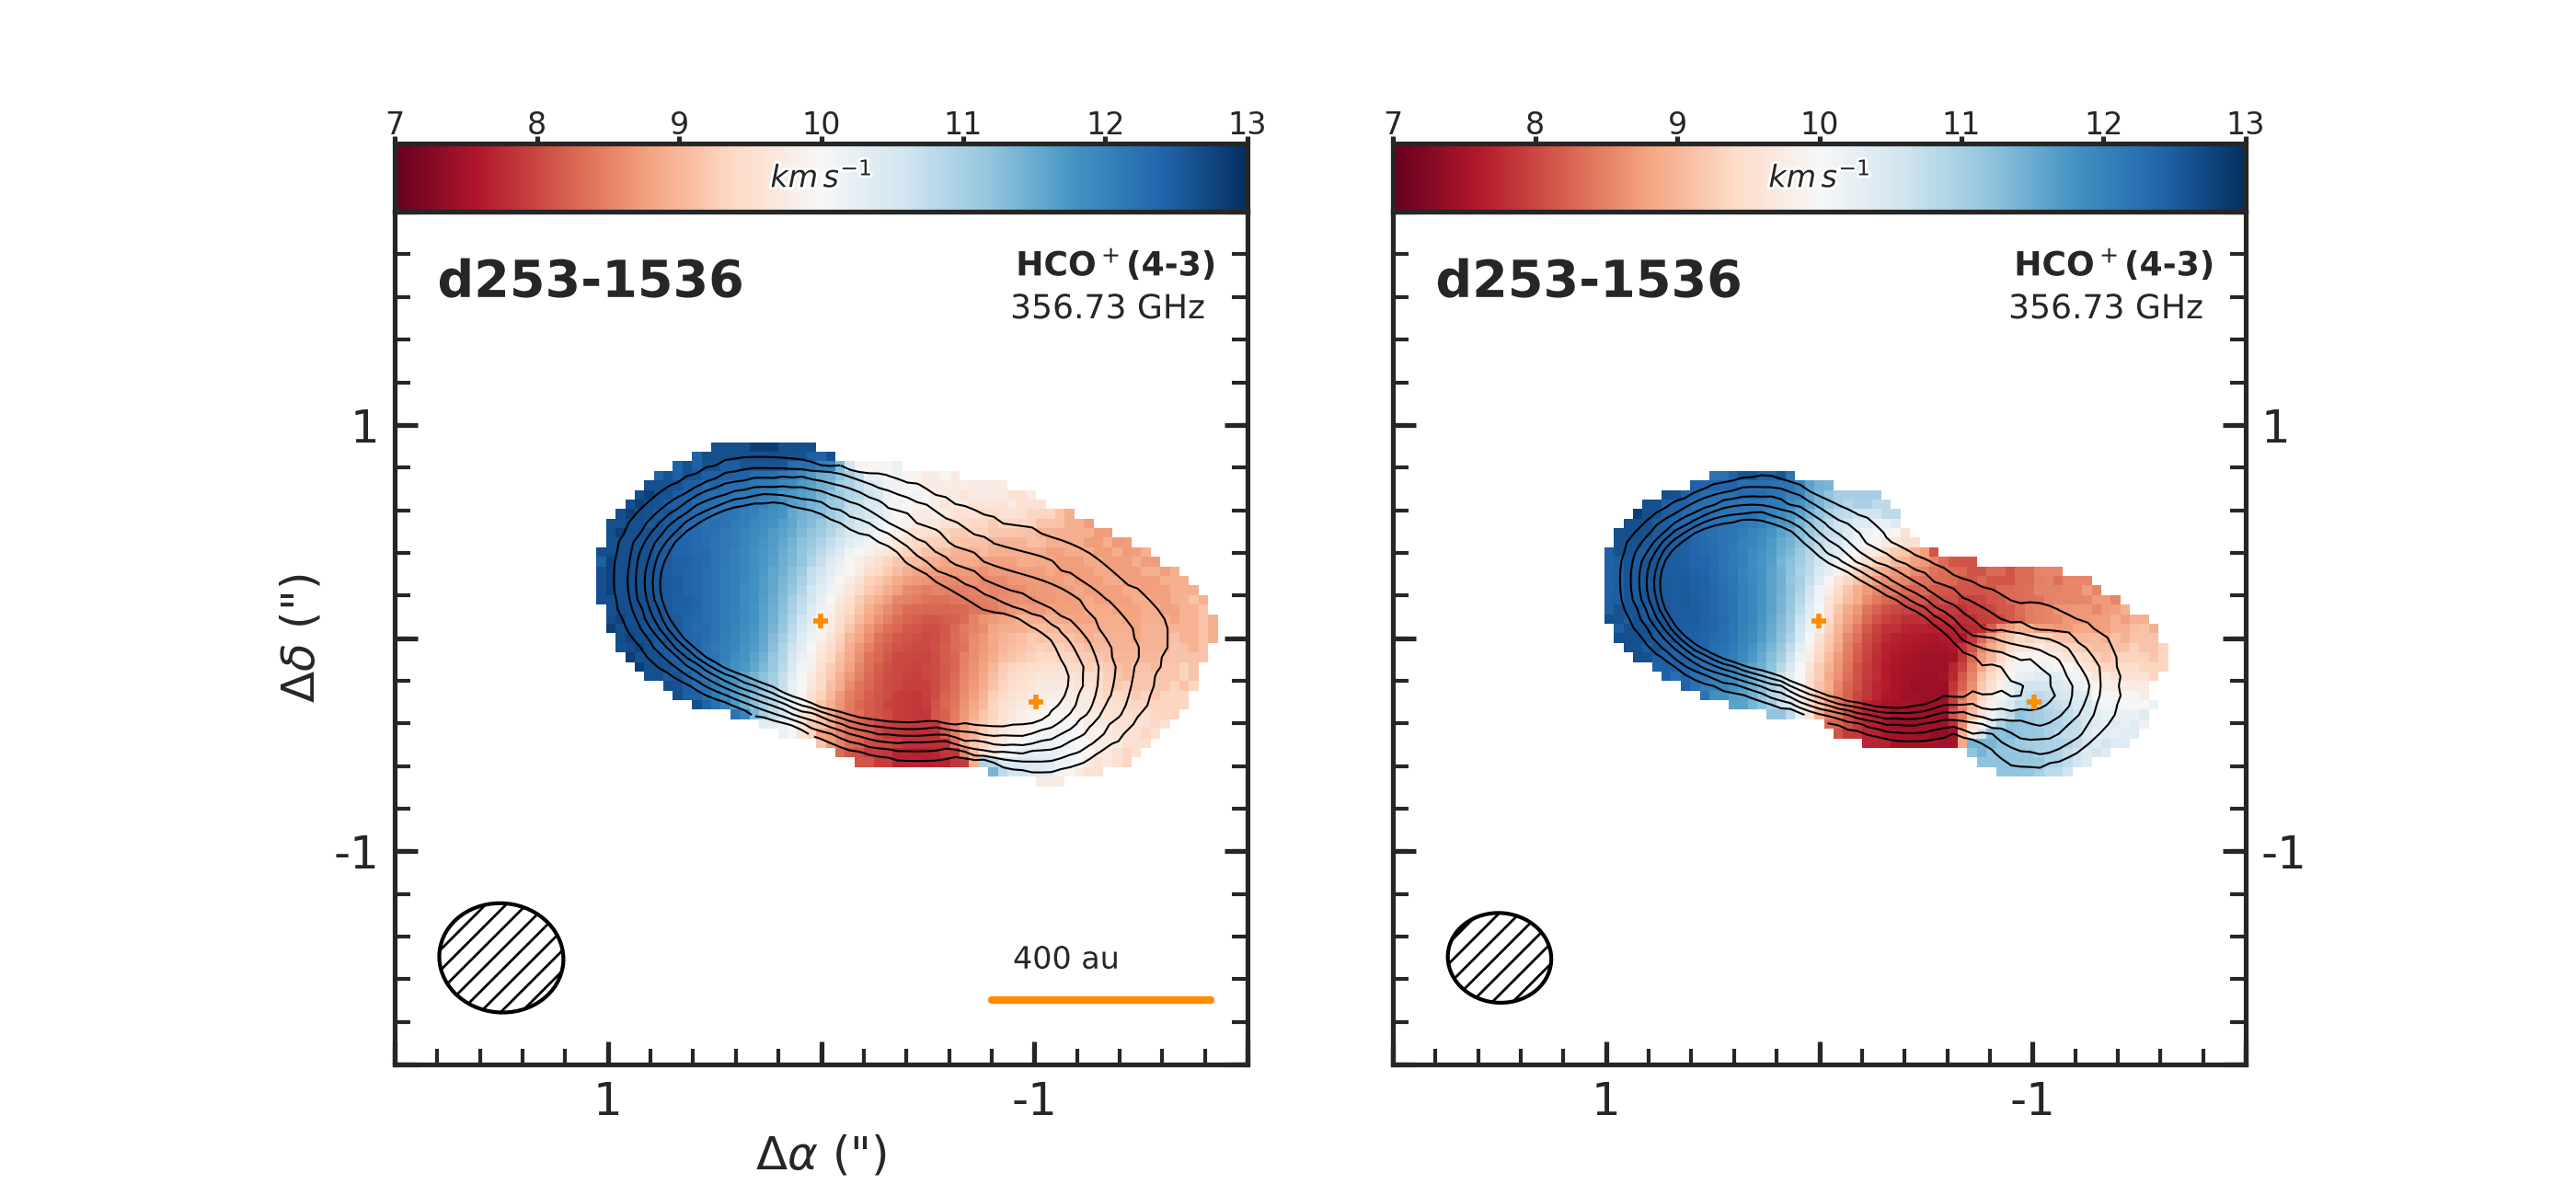
\includegraphics[width=\linewidth]{moment1_hco-baselines.pdf}}\vfill%
  \subcaptionbox{}{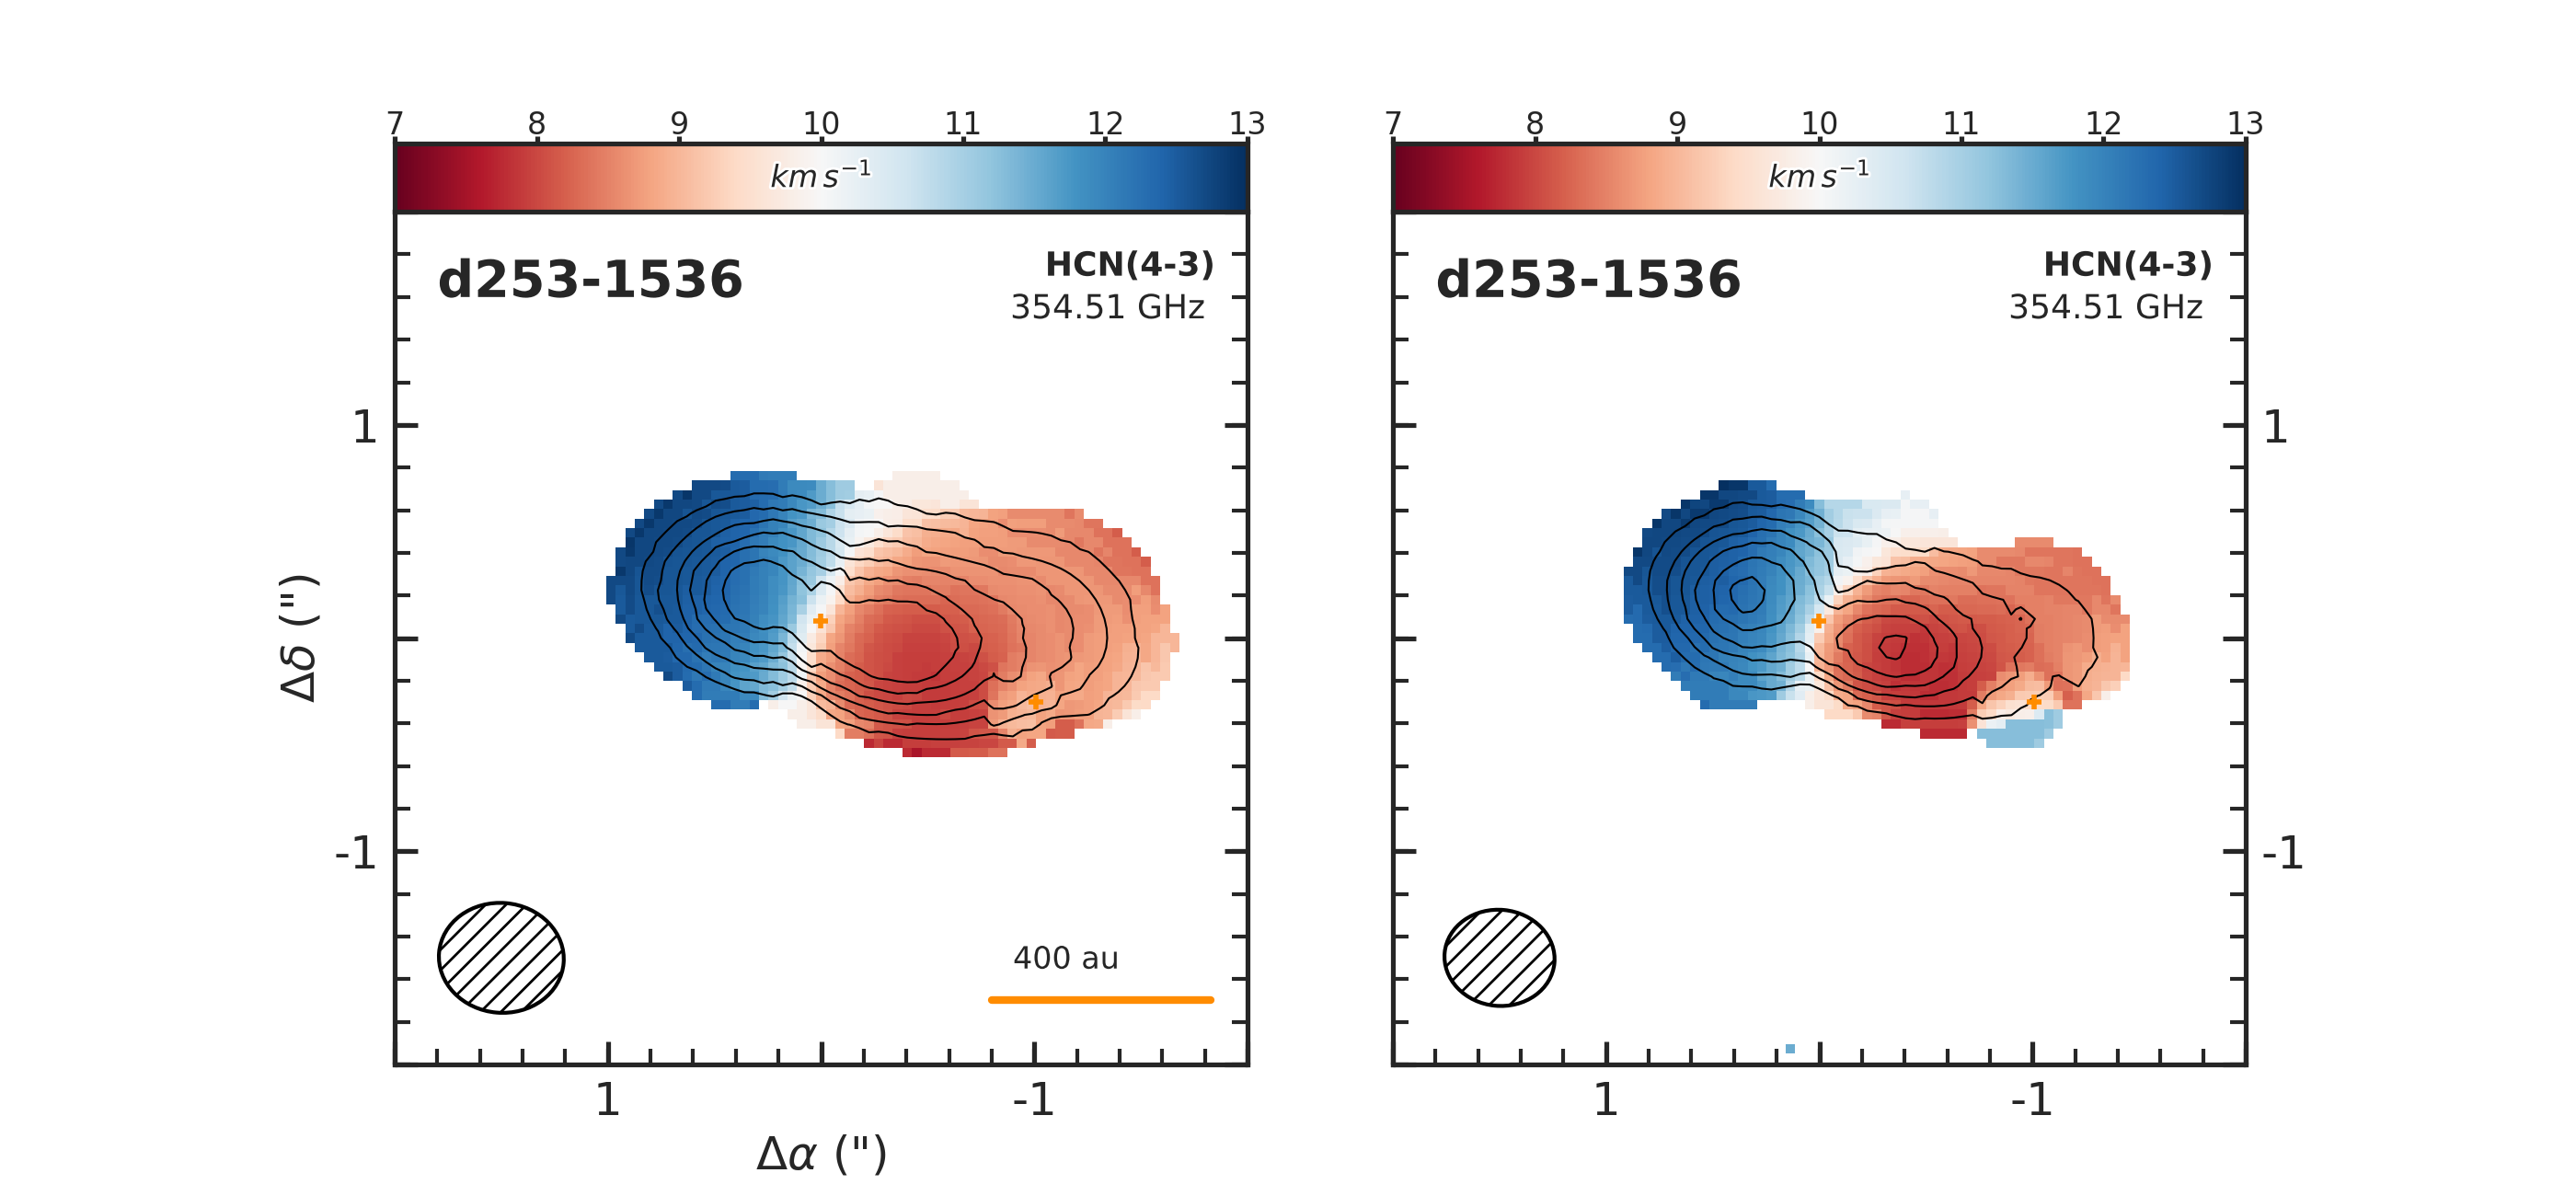
\includegraphics[width=\linewidth]{moment1_hcn-baselines.pdf}}\vfill%
  \hspace*{\fill}%
  \caption{Zeroth (contour) and first (color) moment maps of emission from CO, \hco, and HCN are presented. For each pair, the data is shown without (left) and with (right) baseline cuts implemented according to values given in in Table \ref{tab:baseline_cutting_table}. Since the CS line showed no cloud contamination, we did not cut any baselines from it. Moment-zero contours trace 3, 6, 9...-$\sigma$ flux levels.}
  \label{fig:baseline_cuts}
\end{figure}




\begin{figure}
  \centering
  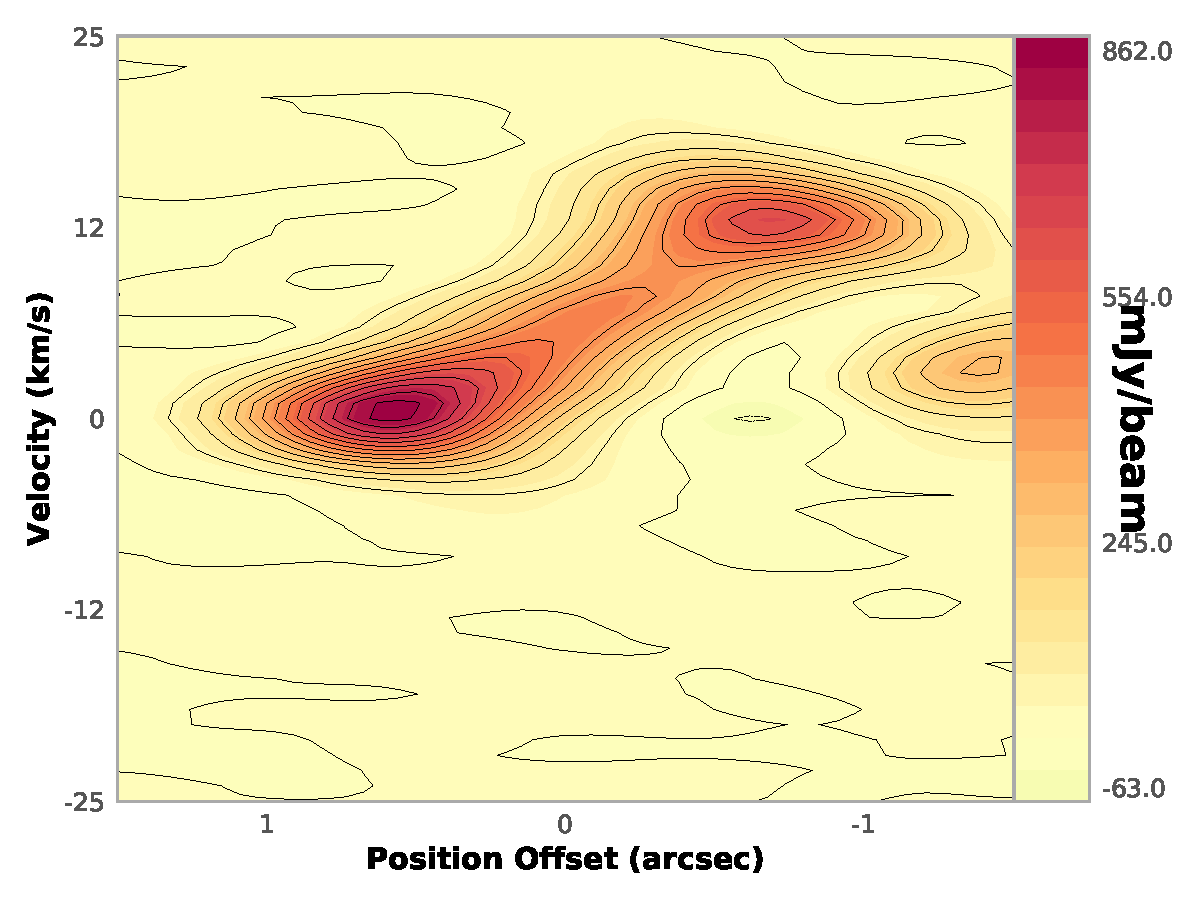
\includegraphics[width=\linewidth]{pvd_A.pdf}
    \captionof{figure}{A PV diagram of disk A's \hco emission, where the x-axis is centered on the disk's position and offset is measured along the disk's position angle. Some asymmetries are readily noticeable, and are likely caused by disk B and excess emission from interactions between the two disks.}
    \label{fig:pv_diag}
\end{figure}

% REWORK: Make this a diptych to show where this slice comes from.





% The End
